\clearpage
\section{Конструкторская часть}

\subsection{Разработка функциональной схемы платы управления}
Плата управления должна выполнять следующие функции:
\begin{itemize}
    \item Генерация управляющего сигнала для двигателя привода нужной мощности
    \item Расчет и выдача управляющего сигналя на усилитель мощности
    \item Получение и обработка сигнала с цифрового датчика угла
    \item Реализация измерения тока в подаваемого на обмотки двигателя
    \item Реализация измерения напряжения в бортовой сети питания
    \item Двусторонний обменa информацией с бортовой ЭВM спутника по бортовой
            сети \textit{RS485}
    \item Формирование напряжений питания для элементов платы управления
\end{itemize}

\subfile{src/pcb_develop/pcb_design.tex}

\newpage
\subsection{Разработка экспериментального стенда}
\label{sec_stand_construction}
\subfile{src/construction/stand_requirements}

\begin{figure}[ht!]
    \centering
    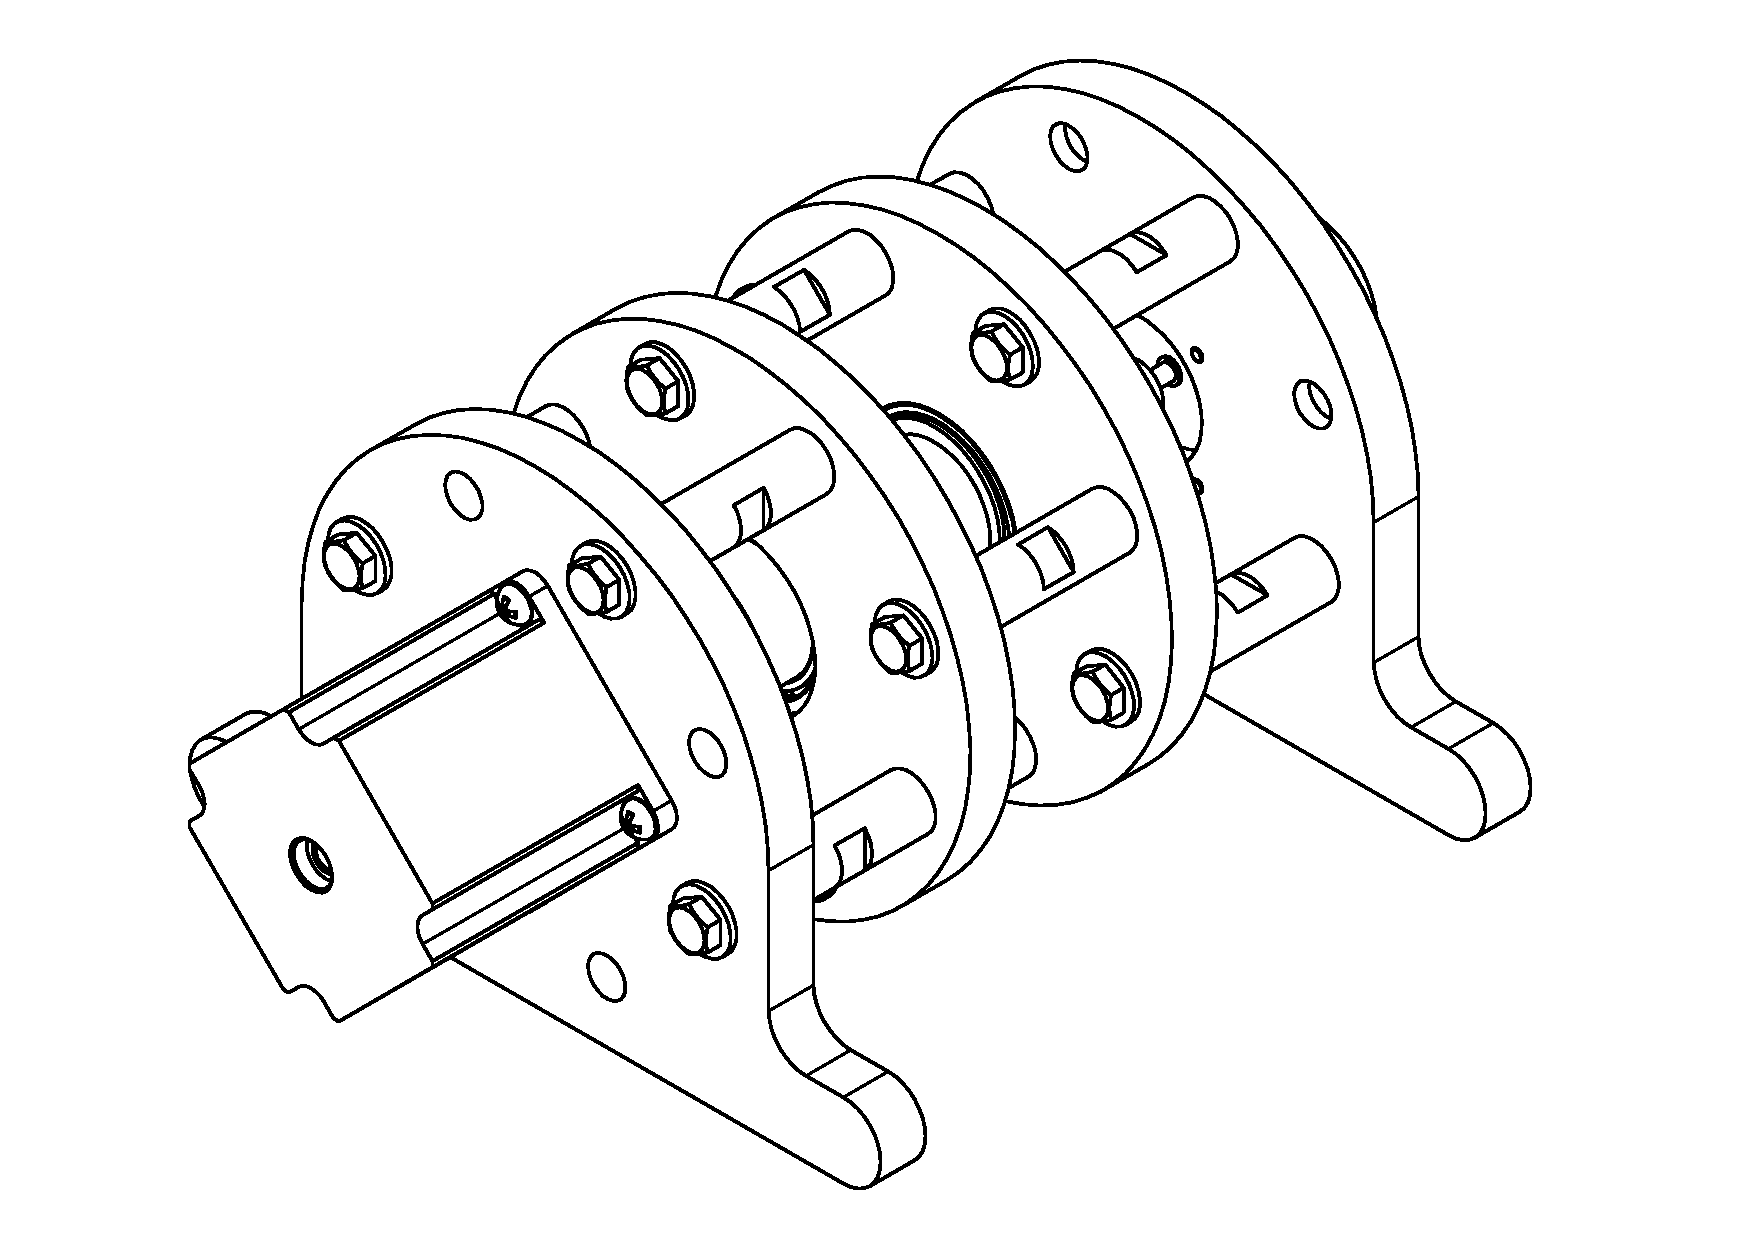
\includegraphics[width=\textwidth, scale=0.6, keepaspectratio]
                    {./src/pictures/stand}
    \caption{Изометрическая проекция экспериментального стенда}
    \label{pic_stand}
\end{figure}

Спроектирован и произведён стенд (рис. \ref{pic_stand}), удовлетворяющий
вышеизложенным требованиям. Стенд предназначен для установки одного датчика угла
и одного двигателя, облатает подшипниковым узлом для избежания чрезмерного
нагружения валов двигателя и датчика. Так же предусмотрена возможность
варьирования момента инерции нагрузки в небольших пределах.

\newpage
\subsection{Разработка программного обеспечения платы управления}
\subfile{src/construction/algo/phase_switch}
